%
% 2
%
\section{\system}
\label{repiano}

{\system}は、
自分の過去の演奏履歴を活用することによって
ひとりでも楽しく演奏を行なうことを可能にするシステムである。
%
過去の演奏を録音しておき、
それを再生しながら新しい演奏を重ねていけば
ひとりでも合奏を行なうことが可能であるが、
現在よく利用されているDTMツールやルーパーの利用はハードルが高い。
{\system}では、
演奏中に
%「録音再生ボタン」
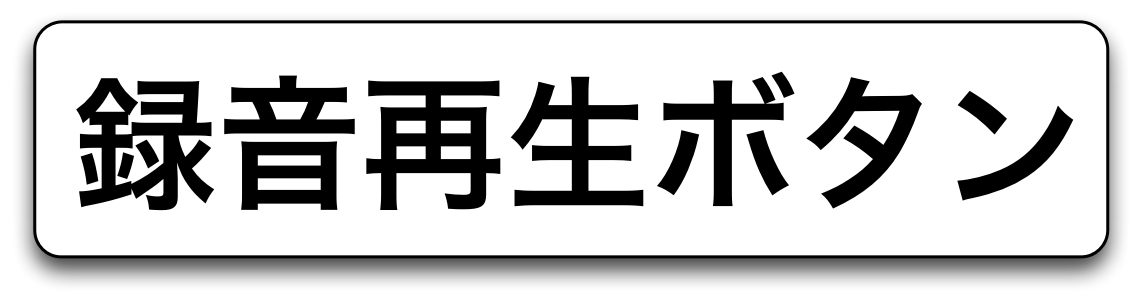
\includegraphics[height=3mm,width=20mm,bb=3 23 360 80]{images/recbutton.png}
を押すだけで
過去の演奏履歴を簡単に再利用することができる。
また、登録した演奏に不具合がある場合は
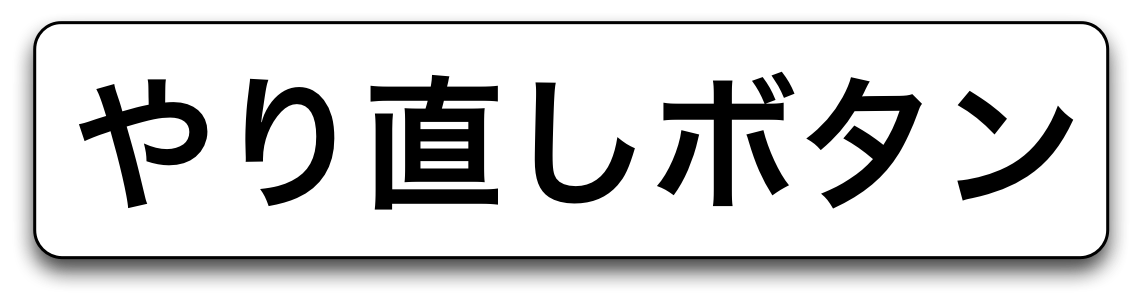
\includegraphics[height=3mm,width=20mm,bb=3 23 360 80]{images/undobutton.png}
ですぐに訂正が可能である。

%2.1
%\subsection{録音再生ボタンによる過去演奏の再生}
% \subsection{\protect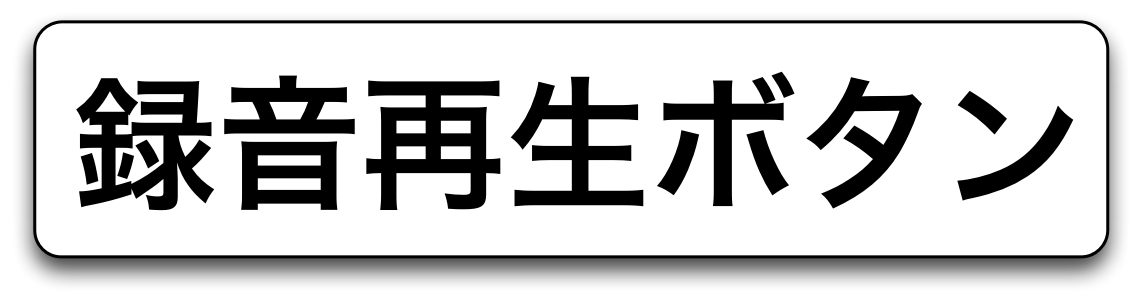
\includegraphics[height=12mm,bb=0 28 360 220]{images/recbutton.png} による過去演奏の再生}
\subsection{\protect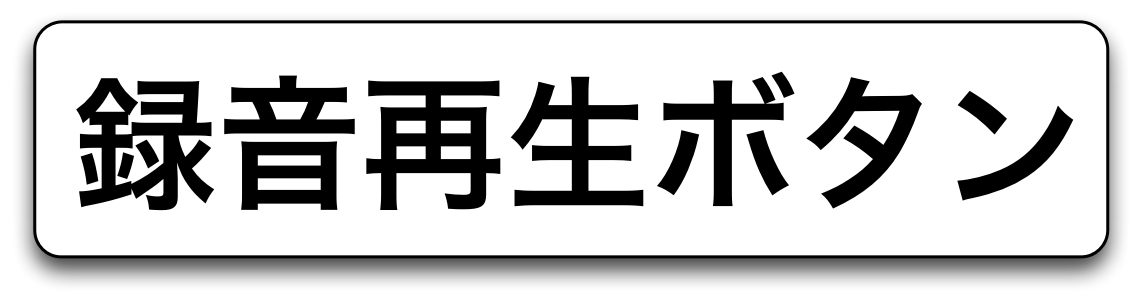
\includegraphics[height=3mm,width=20mm,bb=3 23 360 80]{images/recbutton.png} による過去演奏の再生}
\label{recplaybutton}

{\system}では、演奏中に
% 「録音再生ボタン」
% 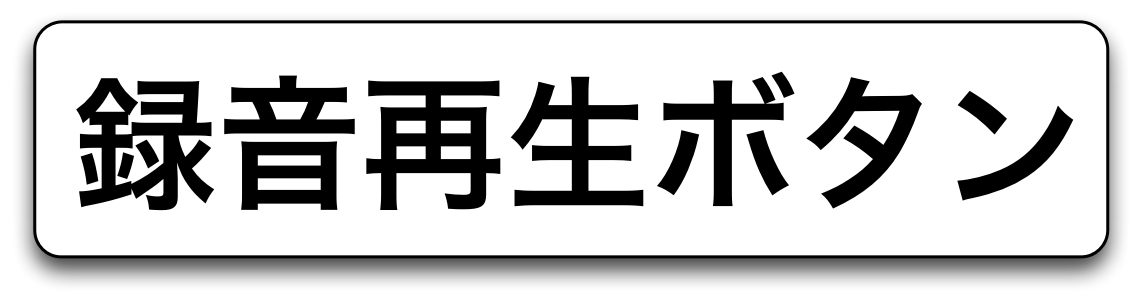
\includegraphics[height=12mm,bb=0 28 360 220]{images/recbutton.png}
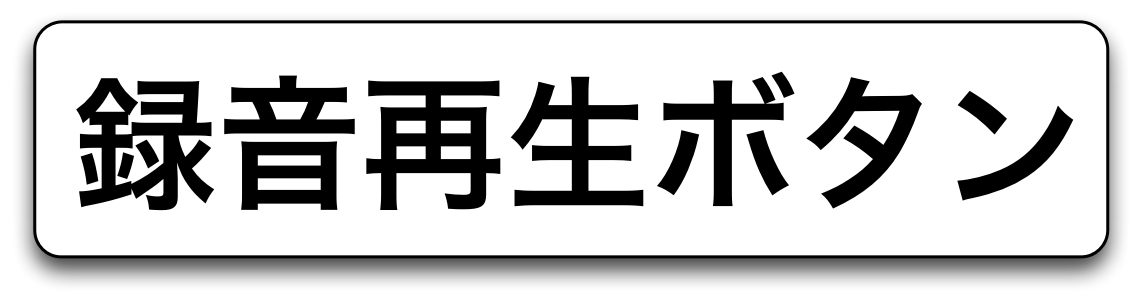
\includegraphics[height=3mm,width=20mm,bb=3 23 360 80]{images/recbutton.png}
を押すことにより
直前の自分の演奏を繰り返し再生することができる。
また、
繰り返し再生中に重ねて演奏したデータを
追加登録することができる。

\subsubsection{単純な過去演奏の再生}

演奏中に
% 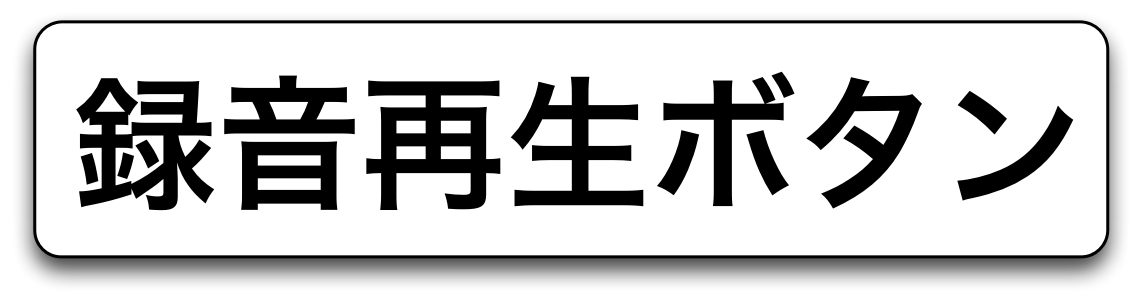
\includegraphics[height=12mm,bb=0 28 360 220]{images/recbutton.png}
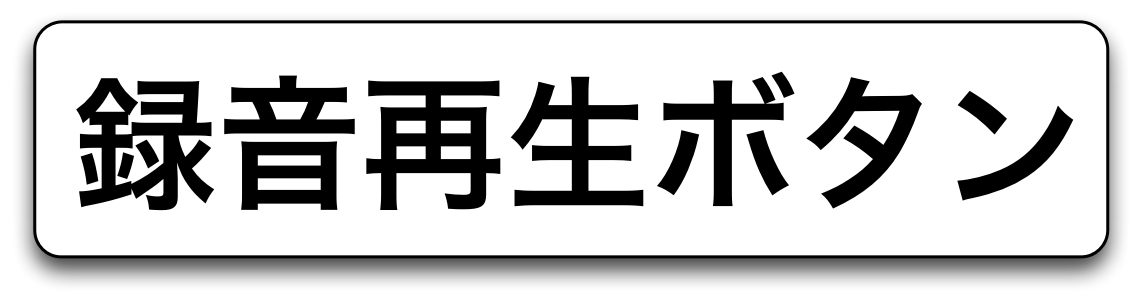
\includegraphics[height=3mm,width=20mm,bb=3 23 360 80]{images/recbutton.png}
% 録音再生ボタン
を押すと、
直前の無音部分から現在までの演奏を登録して
繰り返し再生を行うことができる(\figref{recplay1})。
%
録音開始の操作は不要で、演奏の途中や、
演奏が終わってから登録可能な点が
ルーパーなどの既存のツールとは異なる大きな特徴である。

\subsubsection{二度繰り返された演奏の登録と再生}

同じ演奏を二度繰り返した後で
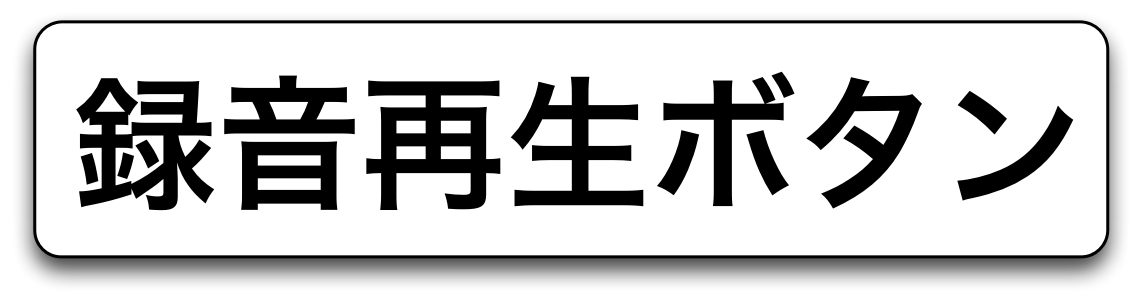
\includegraphics[height=3mm,width=20mm,bb=3 23 360 80]{images/recbutton.png}
% 録音再生ボタン
を押すと、
{\system}は繰り返された部分を自動検出し、
その部分の繰り返し再生を行なう。
\figref{recplay2}の例では、
ボタンを押した時点の直前に「ミソド」が2回繰り返されているため、
「ミソド」が登録されて連続再生される。

この機能は、
テキストエディタ上での操作の繰り返しを検出して
自動実行させることができるDynamic Macro\cite{masui}
の手法を応用したものである。
Dynamic Macroは、
テキストエディタ上で同じ操作を二度繰り返した後で
「繰り返しキー」を押すことにより
繰り返された操作を再実行することを可能にしたものであるが、
{\system}では
同じ演奏を二度繰り返した後で
% 録音再生ボタン
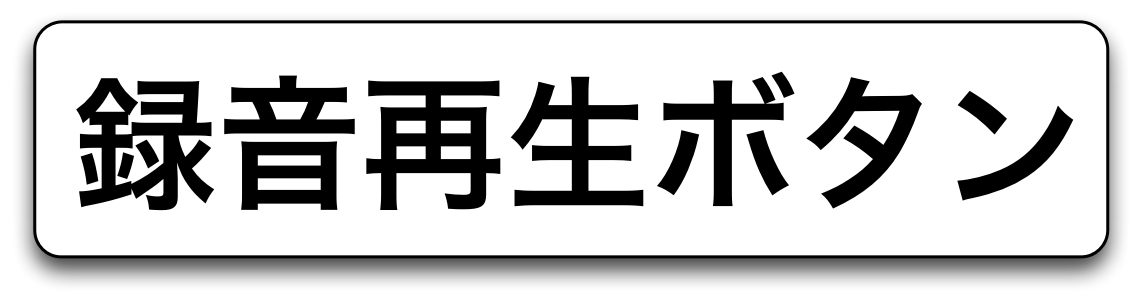
\includegraphics[height=3mm,width=20mm,bb=3 23 360 80]{images/recbutton.png}
を押すことによって
繰り返された部分を登録して連続再生を行うことができる。

\subsubsection{演奏の追加登録}

登録されたフレーズの繰り返し再生中に重ねて演奏を行なうことができるが、
そこで録音再生ボタンを押すとその演奏も新たに登録される(\figref{recplay3})。
この演奏は最初に登録された繰り返しフレーズのタイミングに合わせて記録されるため、
時間が経過してもずれることなく再生され続ける。

\begin{figure}[tb]
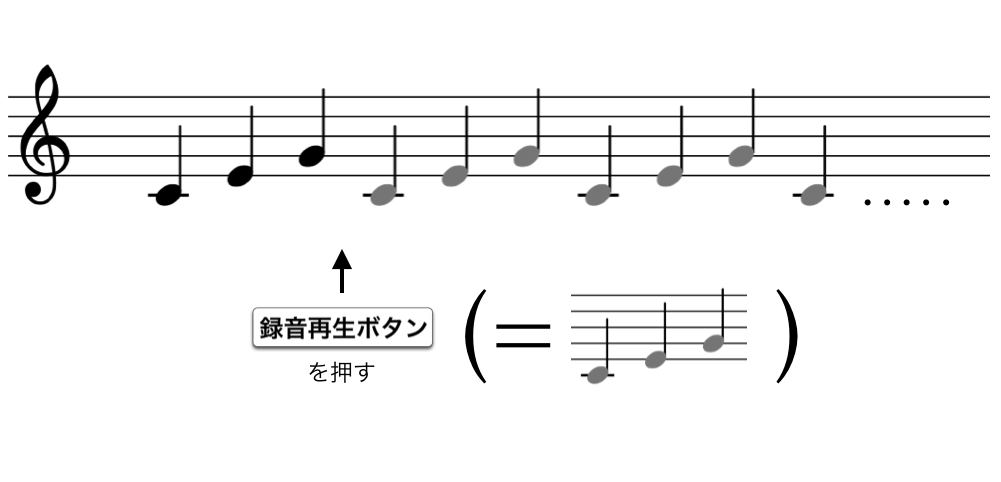
\includegraphics[width=8cm,bb=0 0 1001 482]{images/rp1.png}
\centering
\caption{演奏の登録}
\label{recplay1}
\end{figure}

\begin{figure}[tb]
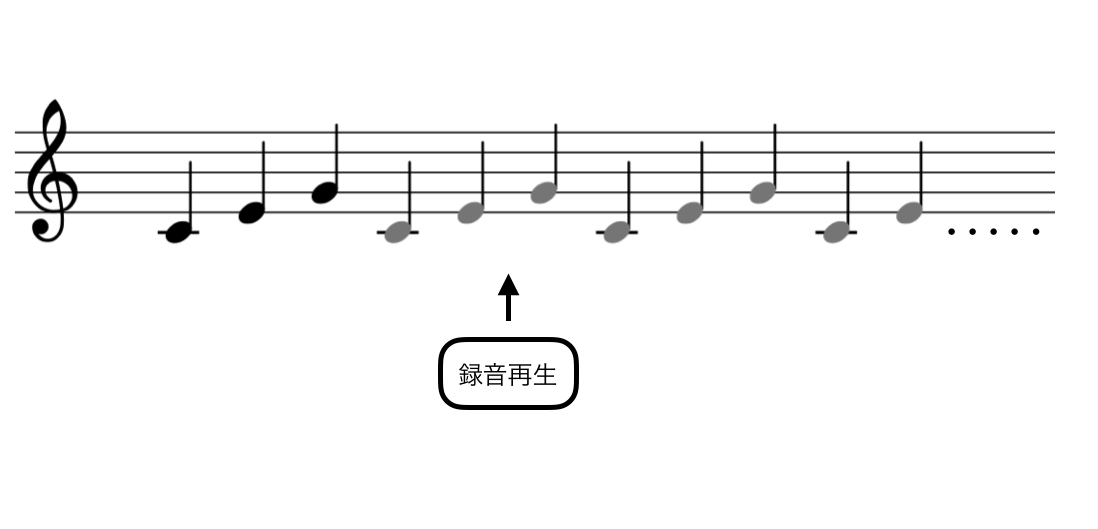
\includegraphics[width=8cm,bb=0 0 1038 532]{images/rp2.png}
\centering
\caption{Dynamic Macroの適用}
\label{recplay2}
\end{figure}

\begin{figure}[tb]
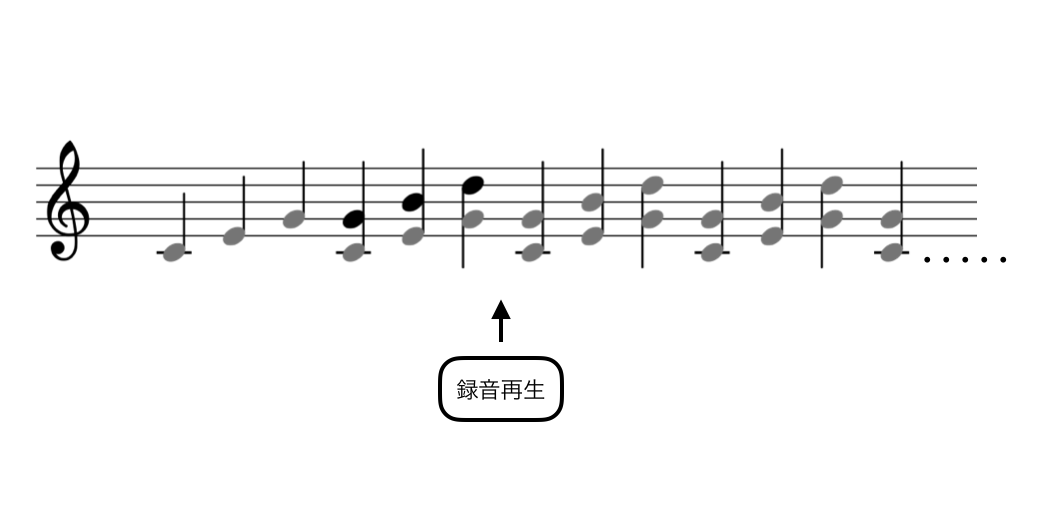
\includegraphics[width=8cm,bb=0 0 1026 544]{images/rp3.png}
\centering
\caption{重ねて演奏を登録}
\label{recplay3}
\end{figure}

\begin{figure}[tb]
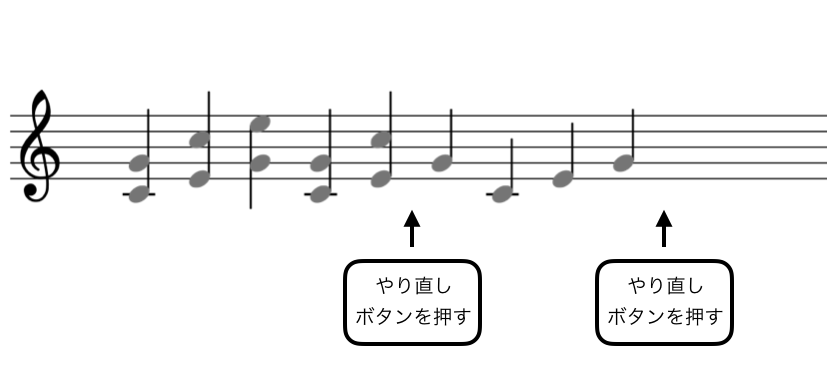
\includegraphics[width=8cm,bb=0 0 1010 440]{images/rp4.png}
\centering
\caption{演奏の取り消し}
\label{recplay4}
\end{figure}

%2.2
%\subsection{やり直しボタン}
\subsection{\protect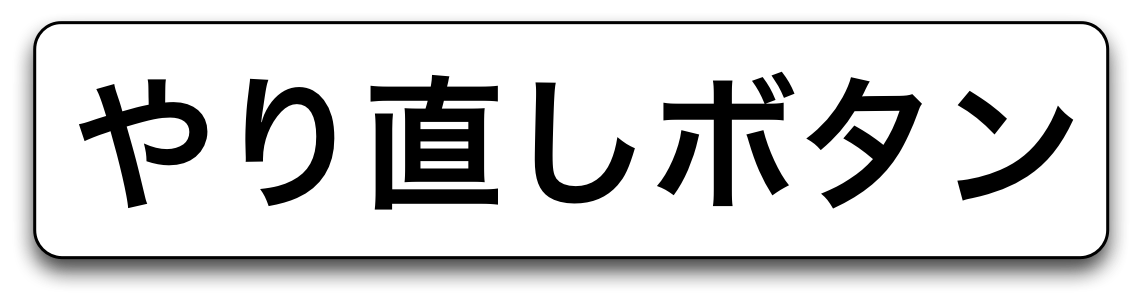
\includegraphics[height=3mm,width=20mm,bb=3 23 360 80]{images/undobutton.png}}

\ref{recplaybutton}で重ねていった演奏を、
新しいものから順に取り消す(\figref{recplay4})。
登録された演奏はそれぞれ独立して管理されているので、
% やり直しボタン
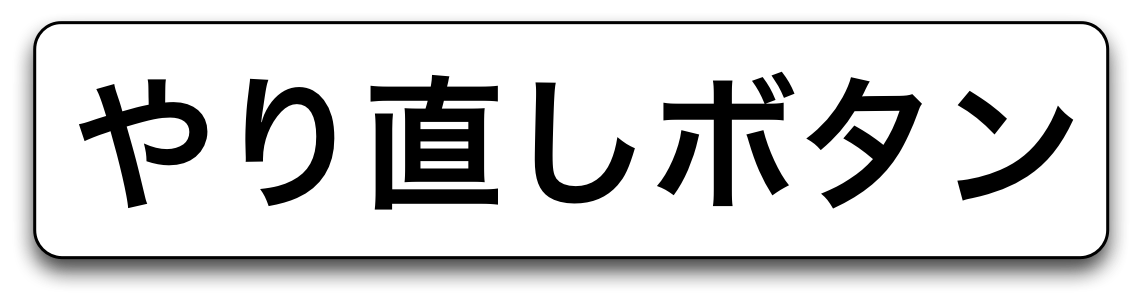
\includegraphics[height=3mm,width=20mm,bb=3 23 360 80]{images/undobutton.png}
によってすぐ以前の状態に戻すことができる。
